\documentclass[12pt]{article}
\usepackage{amsmath,amsfonts,amssymb}
\usepackage{graphicx}
\usepackage{geometry} % Required for customizing margins
\geometry{margin=1in} % Sets 1-inch margins on all sides

\begin{document}

\title{ELCT 331 Control Systems Assignment 1}
\author{Jacob C. Vaught}
\date{Fall 2023 Solutions}
\maketitle

\section*{Problem \#1}
Find the poles and zeros of the following functions (including the ones at infinity, if any). Mark the finite poles with "x" and the finite zeros with "o" in the s-plane.

\begin{enumerate}
  \item \( \frac{10(s+2)}{s^2(s+1)(s+10)} \)
  \item \( \frac{(s+2)}{s(s^2 + 2s + 2)} \)
\end{enumerate}

\subsection*{Solution}

\subsubsection*{(a) Poles and Zeros of \( \frac{10(s+2)}{s^2(s+1)(s+10)} \)}
The given function is:
\[
G(s) = \frac{10(s+2)}{s^2(s+1)(s+10)}
\]
\newline
The zeros are the values of \(s\) that make the numerator zero. In this case, the only zero is at \( s = -2 \), which we mark with an "o" on the s-plane.
\newline \newline
The poles are the values of \(s\) that make the denominator zero. Here, the poles are at \( s = 0 \) with a multiplicity of 2, \( s = -1 \), and \( s = -10 \). We mark these with "x" on the s-plane.
\newline
There are no poles at infinity for this function.
\newline
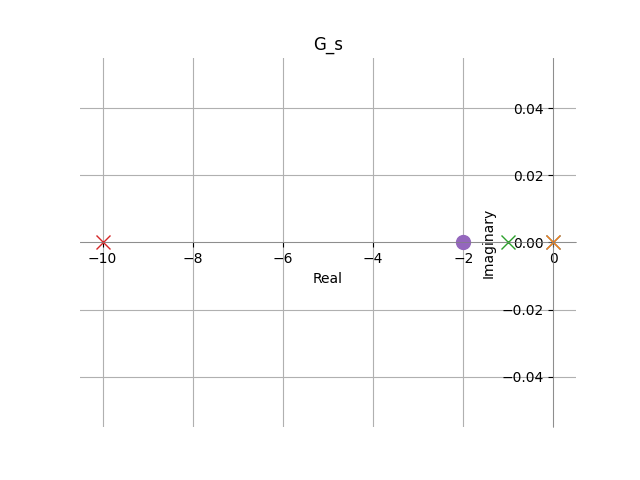
\includegraphics[width=1\textwidth]{G_s.png}

\subsubsection*{(b) Poles and Zeros of \( \frac{(s+2)}{s(s^2 + 2s + 2)} \)}
The given function is:
\[
H(s) = \frac{(s+2)}{s(s^2 + 2s + 2)}
\]
\newline
The zeros are the values of \(s\) that make the numerator zero. Here, the zero is at \( s = -2 \), marked with an "o" on the s-plane.
\newline \newline
The poles are the values of \(s\) that make the denominator zero. For this function, the poles are at \( s = 0 \) and the roots of \( s^2 + 2s + 2 \), which are \( s = -1 \pm j \) (complex conjugate poles). We mark these with "x" on the s-plane.
\newline
There are no poles at infinity for this function.
\newline
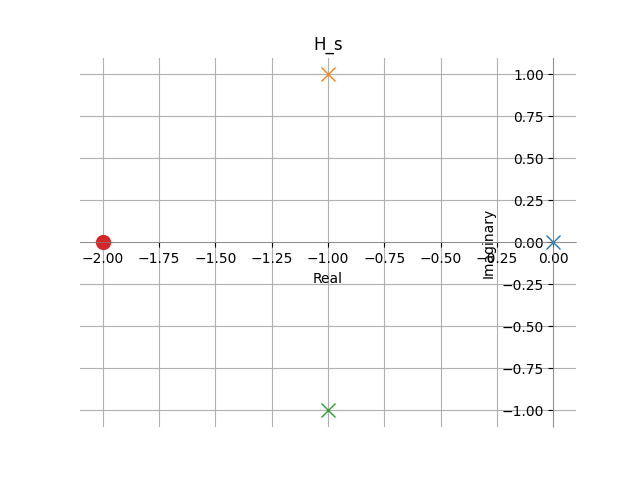
\includegraphics[width=1\textwidth]{H_s.png}

\newpage
\section*{Problem \#2}

\subsection*{Case A}

\begin{itemize}
  \item Simple poles: \(0, -2\)
  \item Poles of order 2: \(-3\)
  \item Zeros: \(-1\)
\end{itemize}

\subsubsection*{Solution}
To write the transfer function, we use the general form:
\[
H(s) = \frac{(s - z_1)(s - z_2) \cdots (s - z_m)}{(s - p_1)(s - p_2) \cdots (s - p_n)}
\]
Given that we have a single zero at \(-1\), the numerator becomes:
\[
(s + 1)
\]
For the denominator, we have simple poles at \(0\) and \(-2\), and a pole of order 2 at \(-3\):
\[
(s - 0)(s + 2)(s + 3)^2 = s(s + 2)(s + 3)^2
\]
Combining these, the transfer function \(H(s)\) for case A is:
\[
H(s) = \frac{(s + 1)}{s(s + 2)(s + 3)^2}
\]

\subsection*{Case B}
\begin{itemize}
  \item Simple poles: \(-3\)
  \item Poles of order 2: \(0, -1\)
  \item Zeros: \(j, -j\)
\end{itemize}

\subsubsection*{Solution}
Again, using the general form of the transfer function, we consider the given zeros \(j\) and \(-j\). The numerator becomes:
\[
(s - j)(s + j) = s^2 + j^2 = s^2 + 1
\]
For the denominator, we have a simple pole at \(-3\) and poles of order 2 at \(0\) and \(-1\):
\[
(s + 3)(s - 0)^2(s + 1)^2 = (s + 3)s^2(s + 1)^2
\]
Combining these, the transfer function \(H(s)\) for case B is:
\[
H(s) = \frac{s^2 + 1}{(s + 3)s^2(s + 1)^2}
\]
\newpage
\section*{Problem \#3}

\textbf{Problem Statement}
Determine if the following systems are stable, marginal, or unstable:
\begin{enumerate}
    \item \( G(s) = \frac{s + 2}{s(s + 1)(s + 3)} \)
    \item \( G(s) = \frac{s(s + 5)}{(s^2 + 1)(s^2 + 3s + 10)} \)
    \item \( G(s) = \frac{s^2 + 10}{(s^2 + 4)^2(s^2 + 3s + 10)} \)
    \item \( G(s) = \frac{s(s + 2)(s + 3)}{(s + 1)(s^2 - 3s + 1)} \)
\end{enumerate}

\subsection*{Solution}

For a system to be stable, all poles of its transfer function must lie in the left half of the complex plane (i.e., have negative real parts).
\newline\newline
\textbf{Part (a)}
\newline
Transfer function \( G(s) = \dfrac{s + 2}{s(s + 1)(s + 3)} \)
\newline
Poles: \(0, -1, -3\)
\newline
All poles are either on the imaginary axis or in the left half of the s-plane. Therefore, the system is marginally stable.
\newline\newline
\textbf{Part (b)}
\newline
Transfer function \( G(s) = \frac{s(s + 5)}{(s^2 + 1)(s^2 + 3s + 10)} \)
\newline
Poles: \(j, -j, -\frac{3}{2} - j\frac{\sqrt{31}}{2}, -\frac{3}{2} + j\frac{\sqrt{31}}{2} \)
\newline
The poles \(j, -j\) are on the imaginary axis. Therefore, the system is marginal.
\newline\newline
\textbf{Part (c)}
\newline
Transfer function \( G(s) = \dfrac{s^2 + 10}{(s^2 + 4)^2(s^2 + 3s + 10)} \)
\newline
Poles: \( -2j, -2j, 2j, 2j, -\dfrac{3}{2} - j\dfrac{\sqrt{31}}{2}, -\dfrac{3}{2} + j\dfrac{\sqrt{31}}{2} \)
\newline
Since two-order poles are on the imaginary axis, the system is unstable.
\newline\newline
\textbf{Part (d)}
\newline
Transfer function \( G(s) = \frac{s(s + 2)(s + 3)}{(s + 1)(s^2 - 3s + 1)} \)
\newline
Poles: \( -1, \frac{3 \pm \sqrt{5}}{2} \)
\newline
One of the poles, \( \frac{3 + \sqrt{5}}{2} \), has a positive real part. Therefore, the system is unstable.
\newpage
\section*{Problem \#4}
Find the Laplace transforms of the following functions. Use the theorems on Laplace transforms, if applicable.
\begin{enumerate}
  \item \( g(t) = 5t e^{-5t} u_s(t) \)
  \item \( g(t) = (t \sin(2t) + e^{-2t}) u_s(t) \)
\end{enumerate}

\subsection*{Solution}

\subsubsection*{(a) Solution for \( g(t) = 5t e^{-5t} u_s(t) \)}

The Laplace transform is defined as
\[
L\{ f(t) \} = \int_{0}^{\infty} e^{-st} f(t) \, dt
\]
\newline
In this case, \( g(t) = 5t e^{-5t} \). Here \( u_s(t) \) is the unit step function, which is 0 for \( t < 0 \) and 1 for \( t \geq 0 \). Because we're already starting our integral from 0, the unit step function doesn't affect the integral.
\newline \newline
We find the Laplace transform as follows:
\[
L\{ 5t e^{-5t} \} = \int_{0}^{\infty} e^{-st} \cdot 5t e^{-5t} \, dt
\]
\[
= 5 \int_{0}^{\infty} t e^{- (s+5) t} \, dt
\]
After integration by parts, we get
\[
= \frac{5}{(s + 5)^2}
\]
\newpage
\subsubsection*{(b) Solution for \( g(t) = (t \sin(2t) + e^{-2t}) u_s(t) \)}

This is a more complex function, so let's break it down.
\newline
\newline
First, we have \( t \sin(2t) \), and then we have \( e^{-2t} \). We'll take the Laplace transform for each part separately and then sum them up, thanks to the linearity of the Laplace transform.
\newline \newline
\textbf{Laplace Transform of \( t \sin(2t) \)}
\[
L\{ t \sin(2t) \} = \int_{0}^{\infty} e^{-st} \cdot t \sin(2t) \, dt
\]
After a couple rounds of integration by parts, we find:
\[
= \frac{4s}{(s^2 + 4)^2}
\]
\newline \newline
\textbf{Laplace Transform of \( e^{-2t} \)}
\[
L\{ e^{-2t} \} = \int_{0}^{\infty} e^{-st} \cdot e^{-2t} \, dt
\]
\[
= \frac{1}{s + 2}
\]
\newline
Finally, we sum the two transforms to get:
\[
L\{ g(t) \} = \frac{4s}{(s^2 + 4)^2} + \frac{1}{s + 2}
\]
\newpage

\section*{Problem \#5}
Use Laplace transform to solve the following differential equations:
\begin{enumerate}
  \item \( \frac{d^2f(t)}{dt^2} + 5 \frac{df(t)}{dt} + 4f(t) = e^{-2t} u_s(t) \) \\
  Assume zero initial conditions.

  \item \( \frac{d^3y(t)}{dt^3} + 2 \frac{d^2y(t)}{dt^2} + \frac{dy(t)}{dt} + 2y(t) = -e^{-t} u_s(t) \) \\
  Conditions: \( \frac{d^2y}{dt^2}(0) = -1 \); \( \frac{dy}{dt}(0) = 1 \); \( y(0) = 0 \)
\end{enumerate}

\subsection*{Solutions}
\subsection*{(a) Solution for \( \frac{d^2f(t)}{dt^2} + 5 \frac{df(t)}{dt} + 4f(t) = e^{-2t} u_s(t) \)}

The given differential equation is:
\[
\frac{d^2f(t)}{dt^2} + 5 \frac{df(t)}{dt} + 4f(t) = e^{-2t} u_s(t)
\]
\newline
Taking the Laplace transform of both sides gives:
\[
s^2F(s) - 0 + 5sF(s) - 0 + 4F(s) = \frac{1}{s + 2}
\]
\newline
Since the initial conditions are zero, the equation simplifies to:
\[
(s^2 + 5s + 4)F(s) = \frac{1}{s + 2}
\]

\[
F(s) = \frac{1}{(s + 2)(s^2 + 5s + 4)}
\]
\newline
After partial fraction decomposition, we find that:
\[
F(s) = \frac{1}{6(s + 4)} - \frac{1}{2(s + 2)} + \frac{1}{3(s + 1)}
\]
\newline
Taking the inverse Laplace transform, we find:
\[
f(t) = \frac{1}{6}e^{-4t} - \frac{1}{2}e^{-2t} + \frac{1}{3}e^{-t}
\]
\newpage


\subsection*{(b) Solution for \( \frac{d^3y(t)}{dt^3} + 2 \frac{d^2y(t)}{dt^2} + \frac{dy(t)}{dt} + 2y(t) = -e^{-t} u_s(t) \)}
With the initial conditions \( \frac{d^2y}{dt^2}(0) = -1 \), \( \frac{dy}{dt}(0) = 1 \), and \( y(0) = 0 \).

\subsubsection*{Step 1: Laplace Transform}

Taking the Laplace Transform of each term in the differential equation and considering the initial conditions, we have:

\begin{align*}
\frac{d^3y(t)}{dt^3} &\to s^3 Y(s) - s^2 y(0) - s y'(0) - y''(0) \\
2\frac{d^2y(t)}{dt^2} &\to 2(s^2 Y(s) - s y(0) - y'(0)) \\
\frac{dy(t)}{dt} &\to s Y(s) - y(0) \\
2y(t) &\to 2Y(s) \\
-e^{-t}u_s(t) &\to -\frac{1}{s+1}
\end{align*}

\subsubsection*{Step 2: Combining Terms}

Combining these terms, we get:

\[
s^3 Y(s) - s^2 y(0) - s y'(0) - y''(0) + 2[s^2 Y(s) - s y(0) - y'(0)] + s Y(s) - y(0) + 2Y(s) = -\frac{1}{s+1}
\]

\subsubsection*{Step 3: Substitute Initial Conditions}

Substituting the initial conditions \( y(0) = 0 \), \( y'(0) = 1 \), \( y''(0) = -1 \), we simplify the equation to:

\[
s^3 Y(s) - s + 1 + 2[s^2 Y(s) - 1] + s Y(s) + 2Y(s) = -\frac{1}{s+1}
\]

\[
(s^3 + 2s^2 + s + 2)Y(s) = s - 1 -\frac{1}{s+1}
\]

\subsubsection*{Step 4: Solve for \(Y(s)\)}

Simplifying and solving for \( Y(s) \), we get:

\[
Y(s) = \frac{s}{s^3 + s^2 + s + 1}
\]

\subsubsection*{Step 5: Partial Fraction Decomposition}

Performing partial fraction decomposition on \( Y(s) \):

\[
Y(s) = \frac{s + 1}{2(s^2 + 1)} - \frac{1}{2(s + 1)}
\]

\subsubsection*{Step 6: Inverse Laplace Transform}

Taking the inverse Laplace Transform of each term:

\begin{enumerate}
    \item \(\frac{s + 1}{2(s^2 + 1)}\) decomposes into \(\frac{1}{2} \frac{s}{s^2 + 1} + \frac{1}{2} \frac{1}{s^2 + 1}\), corresponding to \(\frac{1}{2} \cos(t) + \frac{1}{2} \sin(t)\) in the time domain.
    \item \(-\frac{1}{2(s + 1)}\) transforms to \(-\frac{1}{2} e^{-t}\) in the time domain.
\end{enumerate}

\subsubsection*{Final \(y(t)\)}

Combining these transforms, we obtain the solution for \( y(t) \):

\[
y(t) = \frac{1}{2} \cos(t) + \frac{1}{2} \sin(t) - \frac{1}{2} e^{-t}
\]
\newpage
\section*{Problem \#6}
\textbf{Problem Statement}
Find the inverse Laplace transforms of the following functions. First, perform partial-fraction expansion on \( G(s) \); then, use the Laplace transform table.

\subsubsection*{Solution}

\textbf{Part (b)}
\newline
Given \( G(s) = \frac{10}{(s + 1)^2(s + 3)} \)
\newline
Partial-fraction expansion yields:
\[
G(s) = \frac{A}{s + 1} + \frac{B}{(s + 1)^2} + \frac{C}{s + 3}
\]
Upon solving for \( A, B, \) and \( C \), we find \( A = -5/2, B = 5, C = 5/2 \).
\newline
The inverse Laplace transform is \( g(t) = -2.5e^{-t} + 5te^{-t} + 2.5e^{-3t} \).
\newline \newline
\textbf{Part (c)}
\newline
Given \( G(s) = \frac{100(s + 2)}{s(s^2 + 4)(s + 1)}e^{-s} \)
\newline
Partial-fraction expansion yields:
\[
G(s) = 100e^{-s} \left( \frac{A}{s} + \frac{B}{s + 1} + \frac{Cs + D}{s^2 + 4} \right)
\]
Upon solving for \( A, B, C, \) and \( D \), we find \( A = 50, B = 20, C = -30, D = 20 \).
\newline
The inverse Laplace transform is \( g(t) = 100(50 + 20e^{-t} - 15cos(2t) + 10sin(2t))u(t-1) \).
\newline \newline
\textbf{Part (d)}
\newline
Given \(G(s) = \frac{2(s + 1)}{s(s^2 + s + 2)}\)
\newline
Partial-fraction expansion yields:
\[
G(s) = \frac{-1.3532}{s} + \frac{(0.1766 + 1.2028i)s + (0.1766 - 1.2028i)}{s^2 + s + 2}
\]
Upon solving for \( A, B, \) and \( C \), we find \( A = -1.3532, B = 0.1766 + 1.2028i, C = 0.1766 - 1.2028i \).
\newline
The inverse Laplace transform is 
\[
g(t) = 1 - e^{-\frac{t}{2}} \left( \cos\left(\frac{\sqrt{7}t}{2}\right) - \frac{3\sqrt{7}}{7} \sin\left(\frac{\sqrt{7}t}{2}\right) \right)
\].


\newpage
\section*{Problem \#7}

\textbf{Problem Statement:}

Given the linear time-invariant systems represented by the following differential equations, find the transfer function \( \frac{Y(s)}{R(s)} \) for each system.

\subsection*{Solutions}

\subsubsection*{For Equation (b)}

The given equation is:
\[
\frac{d^4y(t)}{dt^4} + 10 \frac{d^2y(t)}{dt^2} + \frac{dy(t)}{dt} + 5y(t) = 5r(t)
\]
Applying the Laplace transform, we get:
\[
s^4Y(s) + 10s^2Y(s) + sY(s) + 5Y(s) = 5R(s)
\]
Combining terms, we can express this as:
\[
(s^4 + 10s^2 + s + 5)Y(s) = 5R(s)
\]
The transfer function \( \frac{Y(s)}{R(s)} \) is then:
\[
\frac{Y(s)}{R(s)} = \frac{5}{s^4 + 10s^2 + s + 5}
\]

\subsubsection*{For Equation (c)}

The given equation is:
\[
\frac{d^3y(t)}{dt^3} + 10 \frac{d^2y(t)}{dt^2} + 2 \frac{dy(t)}{dt} + y(t) + 2 \int_0^t y(\tau) d\tau = \frac{dr(t)}{dt} +2r(t)
\]
Applying the Laplace transform, we get:
\[
s^3Y(s) + 10s^2Y(s) + 2sY(s) + Y(s) + 2\frac{Y(s)}{s} = sR(s) + 2R(s)
\]
Combining terms, we can express this as:
\[
(s^3 + 10s^2 + 2s + 1)Y(s) + 2\frac{Y(s)}{s} = sR(s) + 2R(s)
\]
The transfer function \( \frac{Y(s)}{R(s)} \) is then:
\[
\frac{Y(s)}{R(s)} = \frac{s + 2}{s(s^3 + 10s^2 + 2s + 1) + 2}
\]

\subsubsection*{For Equation (d)}

The given equation is:
\[
\frac{d^2y(t)}{dt^2} + \frac{dy(t)}{dt} + 5y(t) = r(t) +2r(t-1)
\]
Applying the Laplace transform, we get:
\[
s^2Y(s) + sY(s) + 5Y(s) = R(s) + 2e^{-s}R(s)
\]
Combining terms, we can express this as:
\[
(s^2 + s + 5)Y(s) = R(s) + 2e^{-s}R(s)
\]
The transfer function \( \frac{Y(s)}{R(s)} \) is then:
\[
\frac{Y(s)}{R(s)} = \frac{1 + 2e^{-s}}{s^2 + s + 5}
\]

\end{document}
